\documentclass[a4paper,10pt, bibliography=totocnumbered]{scrreprt}

\usepackage[utf8x]{inputenc}
\usepackage[english]{babel}

\usepackage{graphicx}
\usepackage{pdfpages}
%\usepackage{subfig}
%\usepackage{microtype}
\usepackage{tabularx}
%\usepackage{amsmath, textcomp}

% Custom packages
\usepackage[numbers]{natbib}
\usepackage{longtable}
\usepackage{ragged2e}
%\usepackage{tikz}
%\usetikzlibrary{positioning}
%\usepackage{pdflscape}
%\usepackage{rotating}

\usepackage{glossaries} 

\usepackage{hyperref}
\hypersetup{
    colorlinks=true,        % false: boxed links; true: colored links
    linkcolor=black,        % color of internal links
%    citecolor=green,        % color of links to bibliography
    citecolor=black,        % color of links to bibliography
    filecolor=magenta,      % color of file links
    urlcolor=blue           % color of external links
}


%% Title Page
\makeatletter
\renewcommand{\maketitle}{\begin{titlepage}
    \vskip 10\p@
    \hbox{
      \vrule depth 0.99\textheight
        \mbox{\hspace{2em}}
      \vtop{
        \vskip 10\p@
        \hspace{4pt}
        \vskip 50\p@
        \begin{flushleft}
          \Large \@author \par
        \end{flushleft}
        \vskip 50\p@
        \begin{flushleft}
          \huge \bfseries \@title \par
        \end{flushleft}
        \begin{flushleft}
          \Large \bfseries \@subtitle \par
        \end{flushleft}
        \vskip 70\p@
        \begin{flushleft}
          \Large \@publishers \par
        \end{flushleft}
        \vskip 50\p@
        \begin{flushleft}
          \Large \@date \par
        \end{flushleft}
        }}
  \end{titlepage}
}
\makeatother

\author{Author 1, Author n}
\title{Title }
\subtitle{Technical Report}
\publishers{\textbf{Advisor University of Heidelberg}\\ Prof. Dr. Barbara Paech, Astrid Rohmann}
\date{mm dd, year}



% Deutsche Absaetze:
\parindent 0pt
\parskip 12pt

\textwidth145mm
\setlength{\oddsidemargin}{0.7cm}
\setlength{\topmargin}{-0.5cm}
\setlength{\textheight}{22.5cm}

\begin{document}
\maketitle

\begin{abstract}
\section*{Abstract}

Testing is an essential and time-consuming part of any software development.
This work is a collaboration that highlights various approaches to how systematic tests can be created to make this process more efficient, clearer, easier or more successful.
After the introduction for this purpose eight different methods are dealt with in own subchapters.
Each of these chapters deals with the investigated approach, describes the problem, discusses the literature search on the topic, and then compares the approaches found in each case via a synthesis matrix.
The approaches are put into practice using the example of a movie manager.
Subsequently, the topic described in this subchapter is summarized and a statement regarding the usage for a systematic test generation is made. 

The first topic dealt with is \enquote{systematic generation of acceptance tests that are executable with FitNesse}.
It is about generating automatic tests with the tool FitNesse.
This approach tries to solve the difficulties of communication among the participants.
For this purpose several artifacts like the fit tables are created and used.
After the investigation, it is concluded that the approaches can work well depending on the project size and experience, but unfortunately it is highly dependent on the latter in particular. 

The next chapter discusses that it should be possible to generate test cases in early phases of development.
\enquote{Transition systems} can help to derive test cases from specifications.
The approaches examined here offer industry standard solutions, but the capability of generating robustness tests for fault detection is still a weakness.

The third subchapter deals with \enquote{Testing with a timing component}.
The difficulty of integrating individual software components into an overall project is described as a problem.
The aspect particularly considered here is the temporal component, since in many real-time systems the exact time between two instruction executions can lead to different results.
After an analysis, the conclusion is drawn that this is still a rarely used approach with many non-automated working steps. 

In the next chapter, approaches for model-based systems are examined.
First and foremost, these include \enquote{classification trees}.
The goal is to derive automatic test cases based on the requirements and the input parameters of a model.
In conclusion, classification trees are described as well arranged and close to the requirements, but can potentially produce many test cases.
Moreover, it is difficult to apply these approaches to systems without a simulated model.

The fifth subchapter focuses on \enquote{model based testing} and examines approaches to make testing with models better and describes the differences between system models and test models.
After the analysis the difficulties in using the tools given in literature are worked out.
Nevertheless, it is possible to reduce test time and errors by using them. 

The initial problem for the next chapter with \enquote{Testing functional and nonfunctional requirements in User Requirements Notation} is the risk for wrong test cases during manual test creation.
User requirements notation should fulfill requirements during test creation and thus prevent incorrect or incomplete tests.
At the end, the problem is discussed that this approach is largely unexplored.
Provided that one makes the effort to take additional steps in test case generation, one still achieves a better quality.

In \enquote{Testing Non-Functional Requirements with Risk Analysis} the focus is on risk analysis, because it is precisely here that error-prone components can be discovered.
Suitable approaches are then sought.
Among the findings here are the importance of automated tests and that tests for non-functional requirements should have more priority. 

The last chapter describes the \enquote{Testing Non-Functional Requirements with Aspects} and puts thereby in the comparison with the previous section the focus on the \enquote{aspects}.
This is intended to describe system-wide functionalities in order to be able to deal with concerns at system level.
Also here the missing availability of tools and suitable research are criticized.
However, the approaches considered seem promising and should be further refined.

Thus, this joint work addresses the merits and difficulties of various test case generation techniques.
Common problems identified are the lack of availability of tools or research, but in suitable use cases most approaches help in improving or automating the test cases.
A final conclusion on this is drawn at the end of this work.

\end{abstract}

\tableofcontents

\chapter{Introduction}\label{sec:introduction}

% Reviewfragen
% - Weckt die Einleitung das Interesse der LeserInnen am Thema?
% - Enthält die Einleitung eine detaillierte Problembeschreibung
%   der Herausforderungen in der Softwareentwicklung, die mit systematischer
%   Testerstellung adressiert werden sollen?
% - Enthält die Einleitung die wesentlichen Aussagen aus den Einleitungen der einzelnen Kapitel?

% Die Einleitung (1 Introduction) des Berichts soll das Interesse der LeserInnen
% am Thema wecken und die gemeinsamen Grundlagen beschreiben. Sie enthält eine
% detaillierte Problembeschreibung der Herausforderungen in der Softwareentwicklung,
% die durch systematische Testerstellung adressiert werden sollen. Zudem enthält sie
% die wesentlichen Aussagen aus den Einleitungen der einzelnen Kapitel 
\section{Systematic Software Testing}\label{sec:introduction_software_testing}

With the rise of smart gadgets and the Internet of Things, more and more parts of our daily life involve technology.
And the software required to run our smartphones, computers and other gadgets  becomes more complex as more data can be processed.
As software becomes more complex, bugs and even small configuration mistakes can have immense consequences as recent data breaches have shown\footnote{\enquote{235 Million Instagram, TikTok And YouTube User Profiles Exposed In Massive Data Leak}, \url{https://www.forbes.com/sites/daveywinder/2020/08/19/massive-data-leak235-million-instagram-tiktok-and-youtube-user-profiles-exposed/}, last visited on 2021-02-10}.
Furthermore, not testing software can have legal consequences.
If basic security measures are not implemented and tested, businesses may violate the \enquote{General Data Protection Regulation}\footnote{see \url{https://eur-lex.europa.eu/legal-content/EN/TXT/?uri=CELEX\%3A02016R0679-20160504&qid=1614251901149}, last visited on 2021-02-25}
(GDPR) and may have to pay fines.
This is not a hypothetical risk.
The \enquote{GDPR Enforcement Tracker}\footnote{see \url{https://www.enforcementtracker.com/}, last visited on 2021-02-10} lists instances where businesses had to pay fines due to \enquote{Insufficient technical and organisational measures to ensure information security}.

Therefore, proper testing of software becomes more important than ever.
But what is software testing? According to the \enquote{Guide to the Software Engineering Body of Knowledge} (short: SWEBOK), \enquote{Software testing consists of the dynamic verification that a program provides expected behaviors on a finite set of test cases, suitably selected from the usually infinite execution domain.}~\cite{SWEBOK}
This means that it may not even be possible to test every input against the expected output, for example if the input is an infinite data stream.
But also for functionality with a finite set of input data, testing every possible combination may not be feasible.
Software testing can take more time than developing the program under test. Hence, software testing can be tedious, difficult and expensive.
So the question arises how software can be tested in an effective and efficient way.

We need to write tests in a systematic way.
This paper contains 9~articles, % TODO: Hat einer aufgehört?
each describing another approach to systematic software testing.

In \autoref{sec:topic_2} % Fitnesse
we focus on acceptance tests with FitNesse.
Communicating requirements between customers and developers can be difficult.
Whereas natural language can be too ambiguous, code can be too technical.
By using FitNesse, human-readable Fit-Tables which include test steps are created that can be understood by customers. By writing fixture classes, these Fit-Tables can be used to automatically run tests.

But having tests may not be enough.
Which requirement is covered by which test?
Can we be sure that the implementation matches the specification?
Traceability becomes necessary and is required to not loose overview over the tests cases and covered requirements.
This is where
\autoref{sec:topic_3} % Transition System
comes into play with transition systems which can be used to automatically create test paths through the application by using formal specifications.

% Notes: Often specification and implementation does not match; traceability issues: which requirement is covered by which test? Solution: Transition system;

After that,
\autoref{sec:topic_4} % Timing Component
looks into testing with a timing component, since for real-time systems, timing is crucial.
In real-time systems, the exact time between two instructions or variances in the individual execution time can lead to different system reactions and therefore different results.

% The aspect particularly considered here is the temporal component, since in many real-time systems the exact time between two instruction executions or variances in the individual execution time can lead to different results.

% Notes: some times issue can only be found if components are linked together; test with same input but different execution time can lead to different reactions in a real-time system.

Following this,
\autoref{sec:topic_5} % Classiciation Tree
looks into decreasing the number of test cases by using classification trees.
Because testing all possible parameter cases becomes unmanageable very fast, these classification trees offer a great way to reduce the complexity of such parameter constructs.
Furthermore, these classification trees can be used to generate test cases.

% Notes: Testing all possible cases becomes unmanageable very fast.Classification Trees offer an approach to offer an approach to reduce the complexity of such parameter con-structions  and  to  keep  them  clearly  arranged.  Test cases can be generated from CTs

\autoref{sec:topic_6} %TODO % Formal specification
\textit{is missing}
% Noch nicht online

In \autoref{sec:topic_7} %  System models
we then look into testing with systems models which are compared against test models.
It is looked into model based testing and how traceability can be used to increase the probability of finding errors and improve test quality.

% KEIN autoref, da sonst kleingeschrieben
Chapter~\ref{sec:topic_8} % NFR/FR Use Requiremetn
explains why writing manual tests for functional and non-functional requirements can be  not only tedious but error prone due to Copy\,\&\,Paste of errors in test logic.
The section describes how test cases can be automatically created by using the user requirements notation that is used for modeling, analyzing, and controlling the correctness and completeness of functional and non-functional requirements.

Another aspect of testing non-functional requirements can be by using risk analysis.
This is where \autoref{sec:topic_9} %  Risk Analysis NFR
steps in and briefly shows how non-functional requirements can be tested and how risk analysis can be used to prioritize test cases.
The section also shows how architectural non-functional requirements such as code conventions can be tested.
\autoref{sec:topic_10} % NFR Aspects
expands on this topic by introducing aspects and aspect oriented programming to test and verify non-functional requirements such as software memory limits and memory leaks.

Finally, \autoref{chap:conclusion} concludes this paper and summarizes each article.

% die Beschreibung der gemeinsamen Grundlagen unter Nutzung des Glossars
% und der Wissensgebiete aus SWEBOK. Das Kapitel gibt einen Überblick über
% die Struktur des Berichts.
\section{Common Fundamentals}\label{sec:introduction_common_fundamentals}
All chapters build upon a common set of fundamental definitions regarding software testing and requirements.
They are listed and mapped to the individual topics in the glossary section of this report.
It is highly recommended to refer to the glossary before reading a chapter or when ambiguities arise while reading a chapter.
However, since it is quite extensive and also contains more topic-specific definitions, the most important terms are defined hereafter.

Like a part of the entries in the glossary section, we use the SWEBOK in its third version as a basis.
Although this guide is already quite old (at least the original version from 2004), hence not fully compliant with current research results, its 15 knowledge areas and basic definitions of a body of knowledge are still useful for classifying the approaches presented in this report and establish a common set of technical terms.

% KEIN autoref, da sonst kleingeschrieben
Let us begin with requirements.
The corresponding SWEBOK knowledge area is \enquote{Software Requirements}.
Relevant sub chapters are \enquote{Software Requirements Fundamentals} and \enquote{Requirements Validation}.
The guide defines requirements as \enquote{a property that must be exhibited by something in order to solve some problem in the real world. [\ldots]
An essential property of all software requirements is that they be verifiable as an individual feature as a functional requirement or at the system level as a non-functional requirement.
It may be difficult or costly to verify certain software requirements.} \cite{SWEBOK}
This definition already points out the difficulty of verifying requirements that necessitates the use of systematic testing techniques, as explained in Section 1.1.
Moreover, it distinguishes between functional requirements, representing a feature the software is to provide, and non-functional requirements, specifying the extend of quality.
Requirements need to be formulated clearly, unambiguously and quantitatively in order to implement and verify them correctly \cite{SWEBOK}.

For software testing, there is no uniform definition.
Therefore, the guide refers to multiple definitions from cited references.
In essence, software testing is to assure that specified requirements are met by the implementation or, from a different perspective, find errors indicating that a requirement has not been met.
This testing process is performed at different levels, as the requirements definition already touched upon.
The SWEBOK guide distinguishes between three test levels: unit testing, verifying isolated functionalities (mostly functional requirements), integration testing, verifying the correct interaction of components and system testing, verifying the behavior of the entire system (mostly non-functional requirements).
Correspondingly, these levels are distinguished by the object of the test (single module, multiple modules, entire system), called the target of the test, and the purpose, called objective of the test \cite{SWEBOK}.

The guide presents a wide array of testing techniques.
For this report, it is important to take notice of the definition of model-based testing: \enquote{A model in this context is an abstract (formal) representation of the software under test or of its software requirements [...].
Model-based testing is used to validate requirements, check their consistency, and generate test cases focused on the behavioral aspects of the software.}\cite{SWEBOK}
Some of the approaches presented in this report are model based, at least partially.
However, it is not always clear what the actual model is and some authors use the term incorrectly.

\section{Outline}
\label{sec:intruduction1.3}

Following this introduction in \autoref{sec:introduction}, nine individual reports each present two different but related approaches for systematic testing in Chapters 2\,-\,10.
The reports introduce their superordinate topic in Sections X.1, outline the results and execution of a literature search based on a given article in Sections X.2 and describe the given and selected approach in Sections X.3.1 and X.4.1 as well as illustrating them using a common set of given requirements in Sections X.3.2 and X.4.2.
Finally, the approaches are compared using a common set of synthesis questions in Sections X.5 and evaluated in Sections X.6.
Chapter 11 concludes the report.
The glossary and bibliography can be found in Chapters 12 and 13.\\

In the following, the given requirements (\autoref{fig:mm}) and synthesis questions, used for each individual report, are depicted.

\newpage
\textbf{Synthesis questions:}

\begin{enumerate}
	\item Description of the approach (What does the approach do?)
	\begin{enumerate}
		\item Which artifacts and relations between artifacts are used in this approach? Which artifacts are created in the course of the approach? How are the artifacts characterized?
		\item What is required and/or input for the application of the approach?
		\item What steps does the approach consist of? Which information is used in which step and how? What are the results of the individual steps?
	\end{enumerate}
	\item[] 
	\item Benefits of the approach (Whom does the approach help and how?)
	\begin{enumerate}
		\item Which usage scenarios are supported by the approach?
		\item Which stakeholders are supported by the usage scenarios?
		\item Which knowledge areas from SWEBOK can be assigned to the usage scenarios?
	\end{enumerate}
	\item Tool support for the approach (What tool support is available?)
	\begin{enumerate}
		\item What tool support is provided for the approach?
		\item Which steps of the approach are automated by a tool? Which steps are supported by a tool, but still have to be executed manually? Which steps are not supported by a tool?
	\end{enumerate}
	\item Quality of the approach (How well does the approach work?)
	\begin{enumerate}
		\item How was the approach evaluated?
		\item What are the (main) results of the evaluation?
	\end{enumerate}
\end{enumerate}


\newpage
\newgeometry{margin=1cm}
\begin{landscape}

\begin{figure}
	\centering
	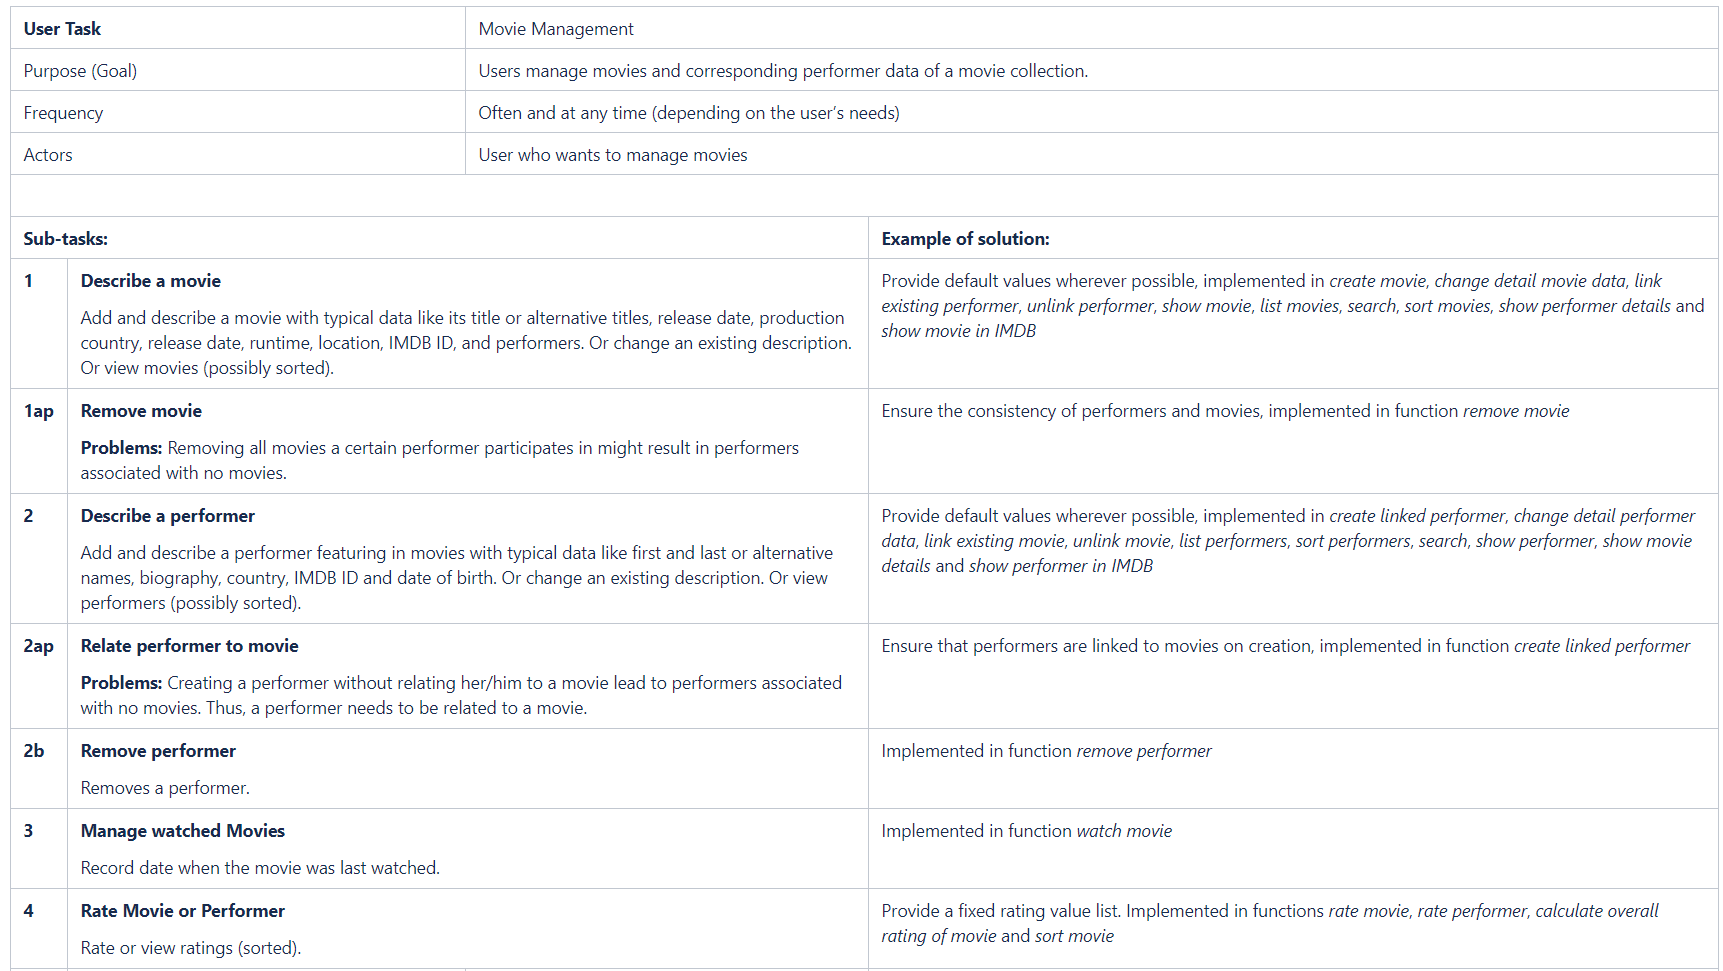
\includegraphics[scale=0.57]{../images/MovieManager.png} 
	\caption{Requirements in User-Task notation for the MovieManager software, an application for managing movie collections.}
	\label{fig:mm}
\end{figure}

\end{landscape}
\restoregeometry



\chapter{Richtiges Zitieren}

1.	Die Seminararbeit ist eine eigenständige wissenschaftliche Arbeit und wird auch nach den Regeln einer wissenschaftlichen Arbeit erstellt (vgl.~\cite{RichtigesZitierenTUDresden}), insbesondere heißt das, dass die Regeln für:
\begin{enumerate}
\item Richtiges Zitieren 
\begin{itemize}
\item Zitierpflicht
\item Zitierregeln
\item Typen von Zitaten
\item Zitierformen
\end{itemize}
\item Literaturangaben 
\item eine gut strukturierte Arbeit 
\end{enumerate}
beachtet und eingehalten werden.




\chapter{Chapter}

Duis porta orci. Integer eu arcu at enim tempus facilisis. Pellentesque dignissim orci sed est. Etiam elementum laoreet mi. Donec nunc sapien, dictum in, tristique sed, aliquam vitae, massa. Morbi magna magna, vestibulum tempor, lobortis non, convallis nec, nibh. In sed nibh. Suspendisse adipiscing dictum pede. Suspendisse non augue. Lorem ipsum dolor sit amet, consectetuer adipiscing elit. Pellentesque lacinia, velit sed commodo convallis, diam dolor consequat ligula, a scelerisque quam neque et purus. Praesent vel augue. Sed lectus leo, dignissim eget, vulputate eu, auctor ut, nulla. Vivamus a quam. Nulla tellus. Pellentesque tempor pulvinar nunc.


\chapter{Conclusion}
Fusce vitae quam eu lacus pulvinar vulputate. Suspendisse potenti. Aliquam imperdiet ornare nibh. Cras molestie tortor non erat. Donec dapibus diam sed mauris laoreet volutpat. Sed at ante id nibh consectetuer convallis. Suspendisse diam tortor, lobortis eget, porttitor sed, molestie sed, nisl. Integer enim nisl, lacinia in, pretium eu, viverra a, odio. Quisque at quam eget risus placerat porttitor. Suspendisse convallis, elit vitae mattis pharetra, orci nisl ultrices sapien, ac interdum metus lorem iaculis diam. Nunc id nunc sit amet nisl tincidunt congue. Curabitur et sapien.

%% Bibliography
\bibliographystyle{plainnat}
%\bibliography{literature.bib}%Bibliography file name

\begin{thebibliography}{9}

\bibitem{KunChen2005} Chen, K, Zhang, W., Zhao, H.: An approach to constructing feature models based on requirements clustering.
In: 13th IEEE International Conference on Requirements Engineering (RE05). pp. 31-40. (2005)

\bibitem{RichtigesZitierenTUDresden} Institut für Geographie   
Lehrstuhl für Allgemeine Wirtschafts- und Sozialgeographie: An Hinweise zum wissenschaftlichen Arbeiten.
\url{http://www.geogr.uni-jena.de/fileadmin/Geoinformatik/Lehre/backup_05_2007/pdf-dokumente/Skript_WissArbeiten.pdf}
\end{thebibliography}

\listoffigures

\listoftables

\end{document}          
